%\documentclass[numsec,webpdf,modern,large,numbered]{oup-authoring-template}
\documentclass[numsec,webpdf,modern,large]{oup-authoring-template}

\graphicspath{{fig/}}

\usepackage{float}
\usepackage{graphicx}
\usepackage{array}
\usepackage{booktabs}
\usepackage{hyperref}
\hypersetup{hidelinks}
\newcolumntype{L}[1]{>{\raggedright\arraybackslash}p{#1}}

\begin{document}

\journaltitle{Bioinformatics}
\DOI{DOI added during production}
\copyrightyear{2026}
\pubyear{2026}
\vol{0}
\issue{0}
\access{Published: Date added during production}
\appnotes{Application Note}

\title[TPSGen]{TPSGen: an integrated framework for motif-conditioned generation and tissue-bias prioritization of tomato promoters}

\author[1,2,3]{Zhoujie Fan}
\author[1,2]{Xiaoyu Wang}
\author[1,2]{Haimeng Zhang}
\author[1]{Hao Meng}
\author[1,3]{Hong Liang}
\author{Tong Zhang}
\author[6]{Huazhu Fu\ORCID{0000-0002-9702-5524}}
\author[7]{Ching-Yu Cheng}
\author{Weihua Pan}
\author[1,2,3,7,*]{Xiaohui Yao\ORCID{0000-0002-8530-7989}}
\author[*]{Cheng Zhao}
\author[1,2,3,8,*]{Shan Cong\ORCID{0000-0002-5981-7678}}

\address[1]{\orgdiv{College of Intelligent Systems Science and Engineering}, \orgname{Harbin Engineering University}, \orgaddress{\street{Harbin}, \postcode{150001}, \country{China}}}
\address[2]{\orgdiv{Qingdao Innovation and Development Center}, \orgname{Harbin Engineering University}, \orgaddress{\street{Qingdao}, \postcode{266000}, \country{China}}}
\address[3]{\orgname{Sanya Nanhai Innovation and Development Base of Harbin Engineering University}, \orgaddress{\street{Sanya}, \postcode{572024}, \country{China}}}
\address[4]{\orgdiv{School of Psychological and Cognitive Sciences}, \orgname{Peking University}, \orgaddress{\street{Beijing}, \postcode{100871}, \country{China}}}
\address[5]{\orgdiv{School of Biomedical Engineering}, \orgname{Hainan University}, \orgaddress{\street{Sanya}, \postcode{572025}, \country{China}}}
\address[6]{\orgdiv{Institute for Infocomm Research}, \orgname{Agency for Science, Technology and Research}, \orgaddress{\street{Singapore}, \postcode{138632}, \country{Singapore}}}
\address[7]{\orgdiv{Department of Ophthalmology, Yong Loo Lin School of Medicine}, \orgname{National University of Singapore}, \orgaddress{\street{Singapore}, \postcode{119228}, \country{Singapore}}}
\address[8]{\orgdiv{Stem Cell and Regenerative Biology, Genome Institute of Singapore}, \orgname{A*STAR}, \orgaddress{\street{Singapore}, \postcode{138672}, \country{Singapore}}}

\corresp[*]{Corresponding authors. Xiaohui Yao (\href{mailto:xiaohui.yao@hrbeu.edu.cn}{xiaohui.yao@hrbeu.edu.cn}); Shan Cong (\href{mailto:shan.cong@hrbeu.edu.cn}{shan.cong@hrbeu.edu.cn})}

\received{14}{9}{2026}
\revised{14}{9}{2026}
\accepted{14}{9}{2026}

\abstract{
% Application Note 的 Summary 要快速说明工具解决什么问题、整合哪些功能、为什么是软件框架；不要展开算法细节，也不要声称新模型或性能最优。
\textbf{Summary:} Engineering tissue-biased promoters in tomato requires coordinated sequence interpretation, candidate construction and tissue-associated prioritization, but these tasks are often distributed across separate resources with heterogeneous interfaces. TPSGen (Tomato Promoter Specificity-guided Generator) is a reproducible, tomato-focused framework that formulates these operations as one standardized promoter-design workflow. It connects motif-aware sequence interpretation, candidate generation and four-tissue score-based prioritization through common inputs, structured outputs and provenance-aware reporting, with package-native and optional model-backed execution routes.\\
% Availability 部分只写实现语言、安装方式、代码位置和许可；这是 Bioinformatics Application Note 审稿人首先检查的软件可用性信息。
\textbf{Availability and Implementation:} TPSGen is implemented in Python and distributed as an installable command-line package. Source code, documentation and example workflows are freely available under the MIT license at \url{https://github.com/Yaolab-fantastic/TPSGen}.\\
\textbf{Contact:} \href{mailto:xiaohui.yao@hrbeu.edu.cn}{xiaohui.yao@hrbeu.edu.cn}; \href{mailto:shan.cong@hrbeu.edu.cn}{shan.cong@hrbeu.edu.cn}.\\
\textbf{Supplementary information:} Supplementary data are available at \textit{Bioinformatics} online.
}

\keywords{tomato promoter engineering, motif-conditioned generation, tissue-bias prioritization, reproducible software, synthetic biology}

\maketitle

\section{Introduction}

Precise regulation of gene expression is essential for plant synthetic biology and crop engineering, where promoter choice and promoter engineering provide a means to control transgene activity with improved spatial specificity \citep{Peremarti2010,Amack2020,Cazier2021}. Computational approaches can facilitate promoter engineering by enabling regulatory sequence interpretation, activity modeling and candidate sequence design \citep{Avsec2021,Washburn2019,Kotopka2020,Zhang2023}. However, these capabilities are frequently implemented as separate tools or task-specific workflows, limiting their integration into reproducible promoter engineering pipelines.


Recent advances in regulatory sequence modeling have enabled diverse computational strategies for promoter analysis, including motif-based interpretation \citep{Lescot2002,Sandelin2004,Fornes2020}, promoter activity modeling \citep{Avsec2021,Washburn2019,Zhang2023}, and synthetic promoter design or regulatory-variant generation \citep{Kotopka2020,Yang2021}. Nevertheless, researchers often need to combine heterogeneous software components, input formats, and analysis procedures when moving from promoter characterization to candidate design. This fragmentation creates practical challenges for reproducibility, software accessibility, and systematic evaluation of computationally designed promoter candidates, particularly in crop-specific applications such as tomato promoter engineering \citep{Sato2012}.
In practice, tissue-associated scoring, candidate generation and post-design sequence-quality checks are also often handled as separate steps, making it difficult to inspect designed promoter candidates within a single shared result schema.

Recent software-focused Application Notes have likewise emphasized installable implementations, standardized interfaces, cross-step workflow integration and reproducible reporting rather than the introduction of a new algorithmic architecture \citep{Lanau2025,RuzJurado2026}. These precedents motivate the framework-oriented presentation adopted here: the contribution of TPSGen is an application workflow that makes complementary promoter-design operations accessible through one reproducible interface, while the underlying sequence-modeling methods are established methods cited separately.

% 中文注释：引言第三段给出本文贡献。正确写法是“reproducible Python framework / workflow / CLI / reporting”，不要写“novel architecture”“state-of-the-art model”。这段要锁定软件发布定位。
Here, we present TPSGen, a reproducible Python framework for motif-aware generation and tissue-bias prioritization of tomato promoter candidates. TPSGen formulates promoter design as a continuous workflow: input sequences are validated and interpreted, sequence evidence is used to constrain candidate construction, and the resulting candidates are scored across four tomato tissues and ranked using a target-bias measure. Package-native deterministic modules provide an immediately executable route, while optional model-backed routes extend sequence evidence and conditional generation. This organization turns complementary computational operations into a single user-facing application with shared input/output schemas, structured reports and provenance records.

\begin{figure*}[t]
\centering
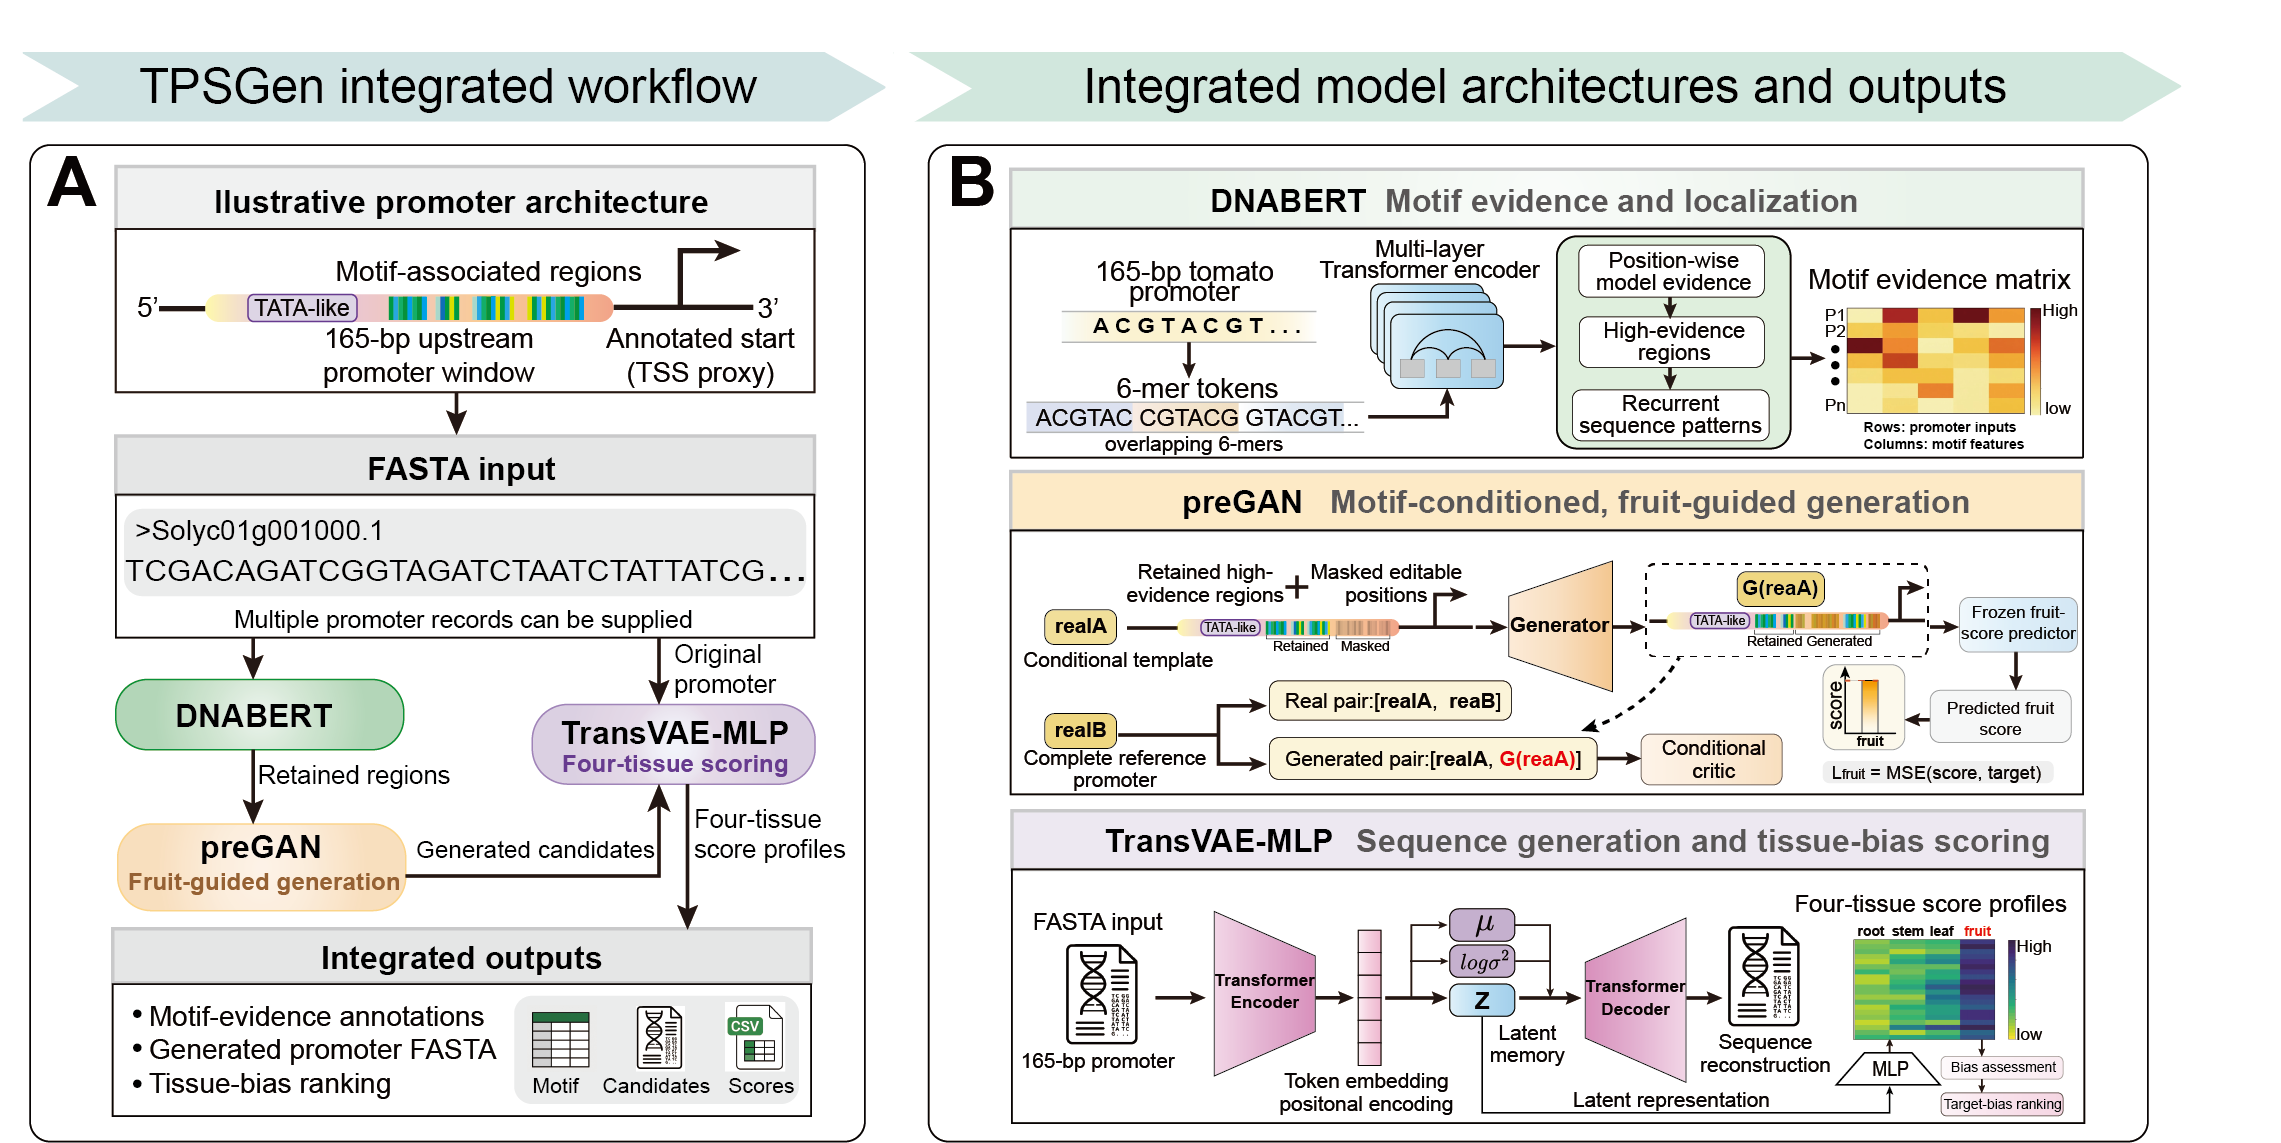
\includegraphics[width=\textwidth]{framework_v2.png}
% 中文注释：主图图注要让 reviewer 快速理解软件输入、核心模块、输出和 retained reference 的边界。D panel 不能写成模型 benchmark，只能写 reproducibility/reference。
\caption{Overview of TPSGen. (A) One or more 165-bp tomato promoter sequences are supplied in FASTA format. Package-native motif annotations or optional DNABERT-derived evidence support motif-aware candidate construction, after which the original and designed sequences can be evaluated using four tissue-associated scores. The workflow reports motif evidence, candidate promoter sequences and tissue-bias rankings. (B) Integrated model architectures and representative outputs. DNABERT converts promoter sequence context into overlapping 6-mer tokens and derives position-wise model evidence and recurrent sequence patterns. When a compatible checkpoint is supplied, preGAN combines retained high-evidence regions with masked editable positions and a frozen fruit-associated predictor to generate conditional candidates. The TransVAE-MLP adapter encodes promoter sequences into a latent representation and uses an MLP to produce root-, stem-, leaf- and fruit-associated scores for bias assessment and candidate ranking. Backend choices and checkpoint use are recorded in the run provenance. All score and generation outputs are computational results and do not by themselves establish experimentally validated tissue specificity.}
\label{fig:framework}
\end{figure*}

\section{Implementation}

TPSGen is a modular Python command-line framework that standardizes tomato promoter design from input sequence to ranked candidates. A multi-record FASTA input is validated, interpreted, used for candidate construction and summarized in a common set of output files. The package-native route runs end-to-end without model retraining; input definitions and model settings are provided in Supplementary Sections S1--S4.

\subsection{Input representation and promoter processing}

The primary input is a multi-record FASTA file containing tomato promoter sequences represented as the project-defined 165-bp windows. TPSGen validates sequence length and alphabet, records rejected records and writes a provenance manifest containing the package version, route, seed and input summary. The model-backed routes therefore have an explicit, reproducible input contract rather than accepting arbitrary genomic sequences without qualification.

Promoter interpretation is provided by a transparent package-native motif scanner and an optional DNABERT-based evidence route. The latter processes overlapping 6-mer tokens and reports position-associated evidence and motif summaries \citep{Ji2021}; it is a project-derived inference route rather than a new DNABERT architecture. Both routes expose their results through standardized tables that can be inspected before candidate construction (Supplementary Section S2).

\subsection{Candidate generation and tissue-associated scoring}

TPSGen separates candidate construction from prioritization while exposing both through the same workflow. The default route performs deterministic motif-aware editing by protecting detected motif positions and applying seeded substitutions to editable positions. When a compatible checkpoint is supplied, the optional preGAN route uses masked 165-bp templates and fruit-associated scalar guidance for conditional generation. In both cases, generation denotes computational candidate construction and not experimentally confirmed promoter activity.

For prioritization, the selected scoring backend reports root-, stem-, leaf- and fruit-associated scores and calculates a target-bias margin for ranking. Backend-specific scores are not assumed to share a common calibration; tissue bias is therefore a computational prioritization signal, not TPM or experimentally validated tissue specificity (Supplementary Section S4).

A central function of TPSGen is to generate candidate FASTA records and evaluate them in the same schema as the input promoter. Each candidate is accompanied by its route, seed, protected-region summary, four tissue-associated scores, target-bias margin and quality-control fields. Thus, sequence construction and candidate prioritization remain traceable within one application rather than requiring manual transfer between independent analysis steps.

Structured reports, example inputs, model resources and provenance manifests support reproducible use. The repository documents optional checkpoint-backed routes separately from the package-native workflow and records the selected backend for each run.



\section{Application Example and Reproducibility}

TPSGen was evaluated as a reproducible software workflow rather than as a new machine-learning benchmark. We assessed a fixed package-native run on 40 tomato promoter sequences of 165 bp, generating three candidates per input with a fixed seed and retaining the complete output manifest.

The run produced motif annotations, candidate FASTA sequences, four score fields, quality-control summaries and a provenance report without manual format conversion. Candidates were ranked using the fruit-associated score and target-bias margin; these outputs support computational prioritization only and are not measurements of promoter expression.

The integrated output of this representative run is summarized in Fig.~\ref{fig:main-results}. The figure reports target-oriented score distributions, 4-mer composition, sequence-level diversity and position-wise sequence remodeling for the input promoters and their Rank-1 candidates. These are computational outputs from one reproducible run and are not experimental measurements of promoter activity.

\begin{figure*}[t]
\centering
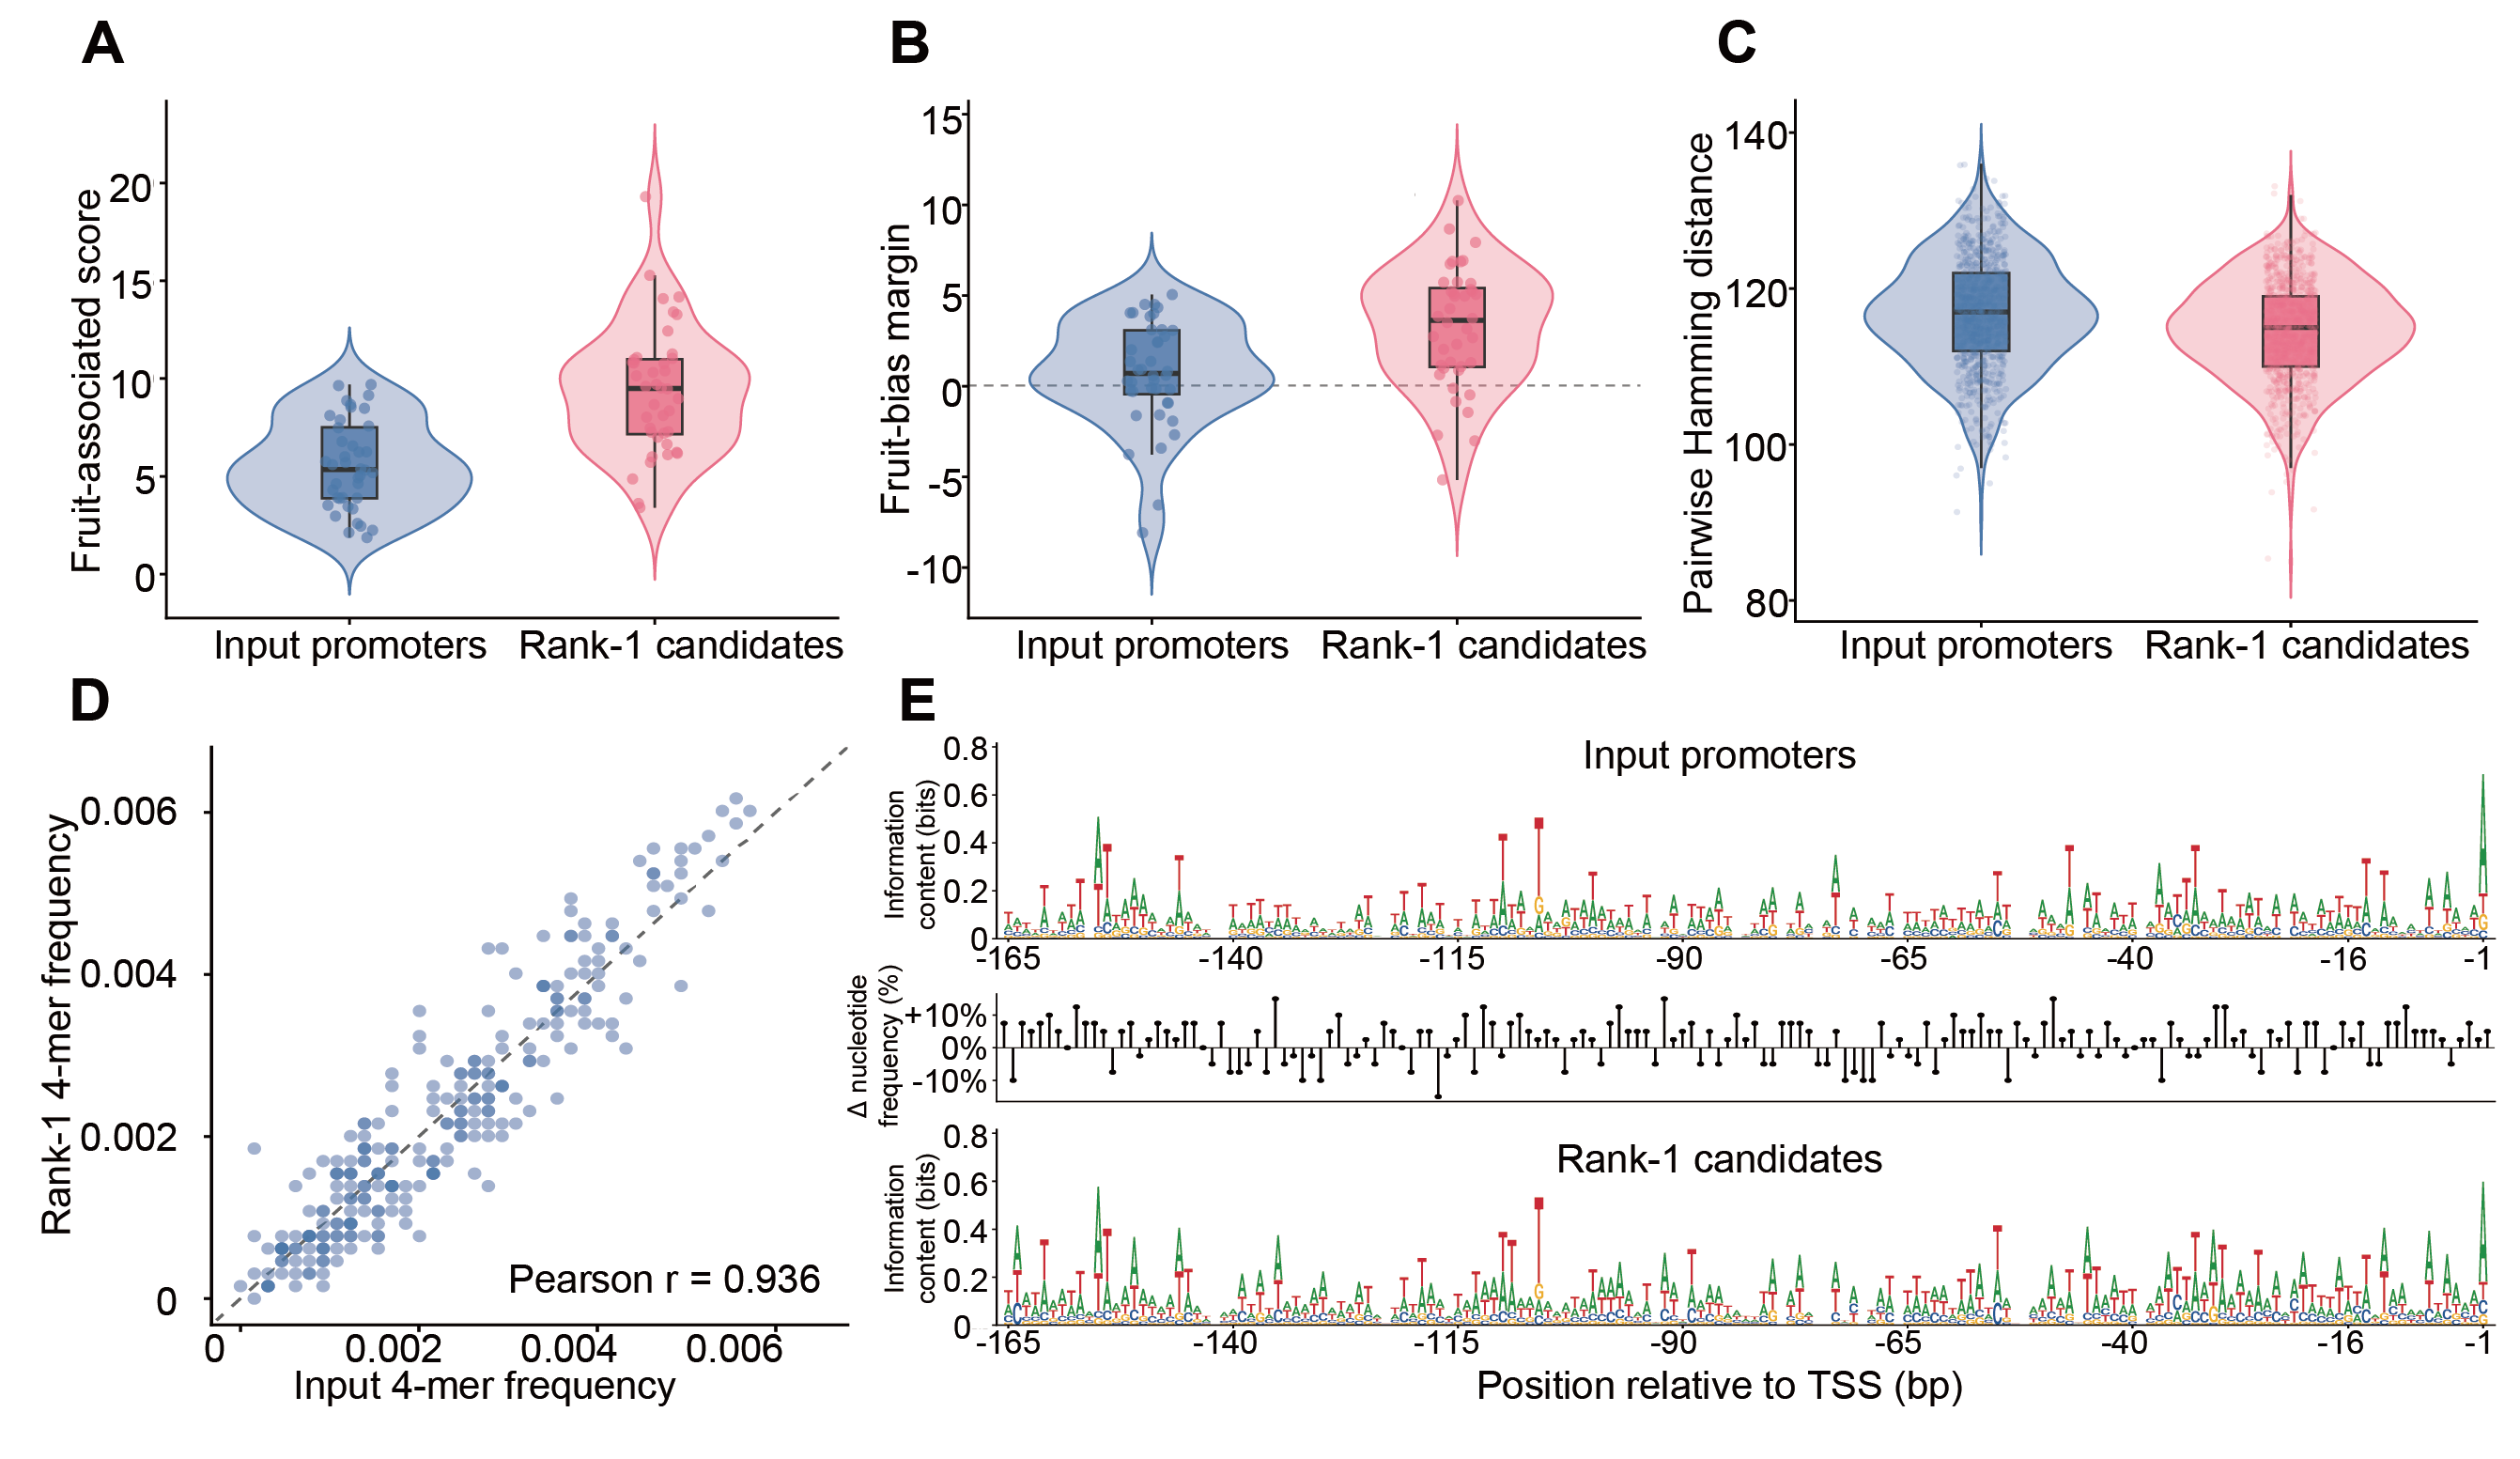
\includegraphics[width=\textwidth]{fig2.png}
\caption{Computational evaluation of TPSGen-designed tomato promoter candidates from a fixed package-native run. (A) Fruit-associated score distributions for input promoters and Rank-1 candidates. (B) Fruit-bias margin distributions, where the dashed line marks zero margin. (C) Pairwise Hamming-distance distributions describing sequence-level diversity within each group. (D) Agreement between aggregated 4-mer frequencies of input promoters and Rank-1 candidates; each point represents one 4-mer and the dashed line denotes equality. (E) Position-wise sequence composition of the input promoters and Rank-1 candidates, with the central track showing the maximum nucleotide-frequency change at each position. All values are computational prioritization outputs and do not establish experimentally validated tissue-specific expression.}
\label{fig:main-results}
\end{figure*}

Historical model-specific results and their provenance are reported separately in the Supplementary Information and are not treated as an independent benchmark of the current package. Together, these results show that TPSGen links promoter characterization, candidate generation and tissue-bias prioritization through a reproducible output schema.



\section{Conclusion}

TPSGen provides a reproducible, tomato-focused application framework that connects promoter interpretation, motif-aware candidate construction and tissue-bias prioritization through standardized interfaces. It is intended to make computational candidates easier to inspect and prioritize for downstream study, while biological validation remains a subsequent experimental step.

\section*{Author contributions}

Z.F. and X.W. led the framework organization, software implementation, computational analyses and manuscript preparation. H.Z., H.M., H.L., H.F. and C.-Y.C. contributed to software, data organization or analysis. X.Y., C.Z. and S.C. provided supervision, scientific interpretation and manuscript revision. All authors reviewed and approved the final manuscript.

\section*{Supplementary data}

Supplementary data are available online at \textit{Bioinformatics} and in the TPSGen repository release.

\section*{Conflict of interest}

The authors declare no conflict of interest.

\section*{Funding}
This work is supported partly by the National Natural Science Foundation of China (62673148), the Hainan Provincial Natural Science Foundation of China (526QN0672, 626MS0266), the Shandong Provincial Natural Science Foundation (ZR2024QF081).

\mbox{}

\section*{Data availability}

Source code, installation instructions, documentation, example tomato FASTA inputs, model definitions, available checkpoint resources and provenance manifests are freely available at \url{https://github.com/Yaolab-fantastic/TPSGen}. The repository also provides the schemas and scripts required to reproduce the package-native example workflow. The tomato reference genome, annotation and expression resources used for the historical model experiments are identified in the Supplementary Information and should be obtained from their original public sources where redistribution is restricted.

\bibliographystyle{oup-abbrvnat}
\bibliography{references}


\end{document}
